\documentclass[aspectratio=169]{beamer}

\usepackage{amsmath}
\usepackage{tikz}

\usetheme{Madrid}
\usecolortheme{seahorse}

\title{Theme Conformance}
\subtitle{Navigation, typography, and template geometry}
\author{}
\institute{}
\date{}

\begin{document}

\section{Foundations}
\subsection{Overview}

\begin{frame}{Typography}
  Body text with inline mathematics $x_1+\lambda=0$.
\end{frame}

\begin{frame}{Columns}
  \begin{columns}[T,totalwidth=\textwidth]
    \begin{column}{.47\textwidth}
      Left column.
    \end{column}
    \begin{column}{.47\textwidth}
      Right column.
    \end{column}
  \end{columns}
\end{frame}

\section{Geometry}
\subsection{Diagram}

\begin{frame}[t]{Theme and drawing geometry}
  \begin{center}
    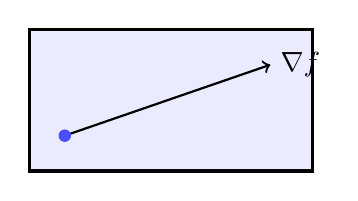
\begin{tikzpicture}[scale=.9]
      \draw[very thick,fill=blue!8] (0,0) rectangle (4,2);
      \draw[->,thick] (.5,.5) -- (3.4,1.5) node[right] {$\nabla f$};
      \fill[blue!70] (.5,.5) circle (2.5pt);
    \end{tikzpicture}
  \end{center}
\end{frame}

\end{document}
